\chapter{Restoration Results and Computational Cost}\label{ch:results}

This chapter reports how well the four trained models restore the 100 DIV2K
validation images, how their quality relates to size and compute, and what
they cost to run. Every model in this chapter was trained once, for 200,000
updates, under the protocol of Chapter~\ref{ch:setup}.

\section{Quantitative Comparison}\label{sec:main-table}

Table~\ref{tab:main} gives the main result. All models start from the same
degraded inputs, with a mean PSNR of 20.99\dB{}.

\begin{table}[htbp]
	\centering
	\caption{Composite restoration on 100 DIV2K validation images after 200,000
	updates. Gain is output minus input PSNR (input 20.992\dB{}). GFLOPs at
	$256\times256$.}
	\label{tab:main}
	\small
	\begin{tabular}{@{}lrrrrrr@{}}
		\toprule
		Method & PSNR$\uparrow$ & Gain & SSIM$\uparrow$ & LPIPS$\downarrow$ & Params & GFLOPs \\
		\midrule
		DnCNN                     & 27.831 & 6.838 & 0.7795 & 0.3242 & 558,403 & 73.43 \\
		FFDNet, blind             & 28.190 & 7.197 & 0.7899 & 0.3176 & 852,108 & 27.89 \\
		FFDNet, oracle$^\dagger$  & 28.240 & 7.247 & 0.7920 & 0.3162 & 852,108 & 27.89 \\
		\fcsg{}                   & 27.243 & 6.250 & 0.7529 & 0.3961 &  97,088 &  9.39 \\
		\bottomrule
		\multicolumn{7}{@{}l}{\footnotesize $^\dagger$Given the true sampled noise level; an upper reference, not a fair competitor.}
	\end{tabular}
\end{table}

\fcsg{} improves the input by 6.25\dB{}, which shows that the network learns
a substantial restoration, but it is the weakest of the four models on all
three metrics. It trails DnCNN by 0.59\dB{} and blind FFDNet by 0.95\dB{}.
The gap is larger in LPIPS than in PSNR: 0.396 against 0.318 for blind
FFDNet, which suggests that \fcsg{} leaves more visible residue than its PSNR
deficit alone would indicate.

The comparison looks different once size and compute are included
(Table~\ref{tab:tradeoff}). \fcsg{} reaches within 0.6\dB{} of DnCNN with
82.6\% fewer parameters and 87.2\% fewer reported FLOPs, and within 1\dB{}
of both FFDNet variants with 88.6\% fewer parameters and 66.3\% fewer FLOPs.

\begin{table}[htbp]
	\centering
	\caption{\fcsg{} relative to each baseline.}
	\label{tab:tradeoff}
	\begin{tabular}{@{}lrrr@{}}
		\toprule
		Compared with & PSNR difference & Fewer parameters & Fewer GFLOPs \\
		\midrule
		DnCNN           & $-0.588$\dB & 82.6\% & 87.2\% \\
		FFDNet, blind   & $-0.947$\dB & 88.6\% & 66.3\% \\
		FFDNet, oracle  & $-0.997$\dB & 88.6\% & 66.3\% \\
		\bottomrule
	\end{tabular}
\end{table}

Two observations about the baselines are worth recording. Blind FFDNet is the
strongest fair model, even though its noise map is a constant and so carries
no information. Its advantage over DnCNN therefore comes from the
architecture, most likely the half-resolution processing that gives each
layer a larger effective receptive field, rather than from noise
conditioning. Second, the oracle map adds only 0.05\dB{} over the blind
constant. Knowing the noise level helps little when blur, resampling and
JPEG artefacts are mixed in, because the map describes only one of the four
corruptions.

Figure~\ref{fig:benchmark} plots the three metrics side by side.

\begin{figure}[htbp]
	\centering
	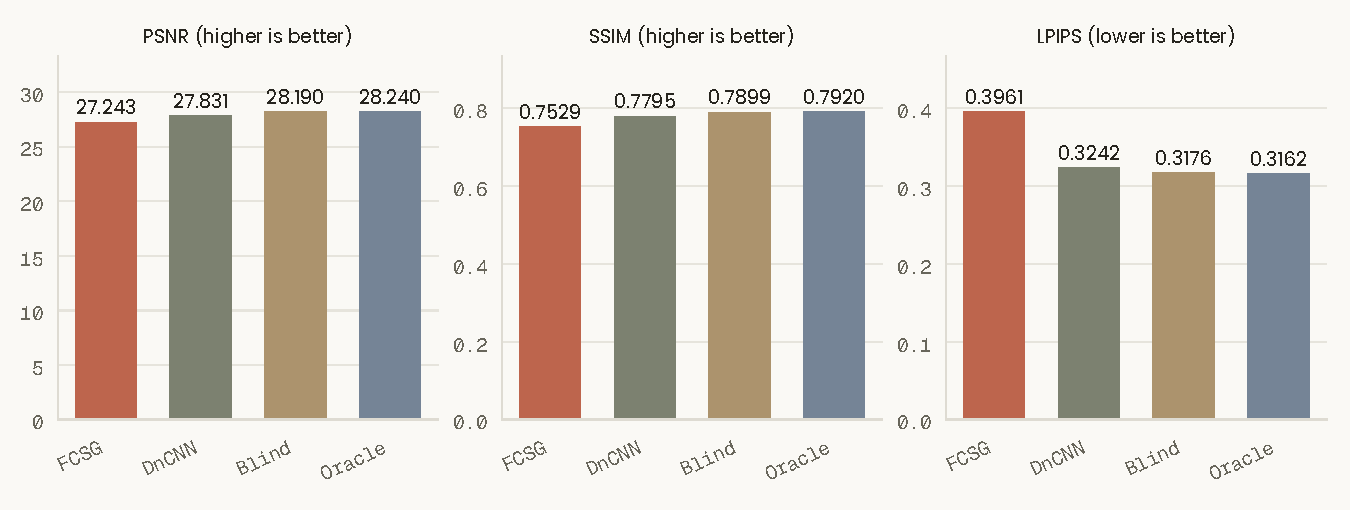
\includegraphics[width=\linewidth]{benchmark.pdf}
	\caption{Mean PSNR, SSIM and LPIPS over the 100 validation images. Each bar
	is one training run.}
	\label{fig:benchmark}
\end{figure}

Each model was trained once with an unfixed seed, so we cannot separate the
effect of the architecture from run-to-run variation. Differences of a few
hundredths of a decibel, such as the one between the two FFDNet variants,
should not be over-read. The gap between \fcsg{} and the baselines is large
enough, and consistent enough across images (Section~\ref{sec:per-image}),
that we do not expect a second seed to reverse it.

\section{Per-Image Analysis}\label{sec:per-image}

Averages can hide a model that wins on most images and loses badly on a few.
Table~\ref{tab:wins} compares \fcsg{} with each baseline image by image.

\begin{table}[htbp]
	\centering
	\caption{Per-image PSNR comparison of \fcsg{} against each baseline, 100 images.}
	\label{tab:wins}
	\begin{tabular}{@{}lccc@{}}
		\toprule
		Compared with & Wins / ties / losses & Mean difference & Range \\
		\midrule
		DnCNN          & 6 / 1 / 93  & $-0.59$\dB & $-2.75$ to $+2.07$\dB \\
		FFDNet, blind  & 0 / 0 / 100 & $-0.95$\dB & $-3.12$ to $-0.04$\dB \\
		FFDNet, oracle & 0 / 0 / 100 & $-1.00$\dB & $-3.48$ to $-0.07$\dB \\
		\bottomrule
	\end{tabular}
\end{table}

The deficit is systematic. Both FFDNet variants beat \fcsg{} on every one of
the 100 images. Against DnCNN, \fcsg{} wins on six images, and on one of them
by 2.07\dB{}, so the two convolutional designs fail in different places.
Image 0801 is an example: DnCNN barely improves it (28.09 to 28.22\dB{}),
while \fcsg{} reaches 29.32\dB{}. Conversely, DnCNN is the only model that
makes some images worse; three of its outputs score below their inputs.

The hardest image for every model is 0828, whose degraded input scores only
17.10\dB{}. \fcsg{} reaches 17.93\dB{} on it and the baselines between 18.61
and 18.83\dB{}. Our experiment does not isolate which of the four sampled
corruptions makes this image so difficult. Figure~\ref{fig:per-image} shows
the paired differences and the error distributions. The full table is in
Appendix~\ref{app:per-image}.

\begin{figure}[htbp]
	\centering
	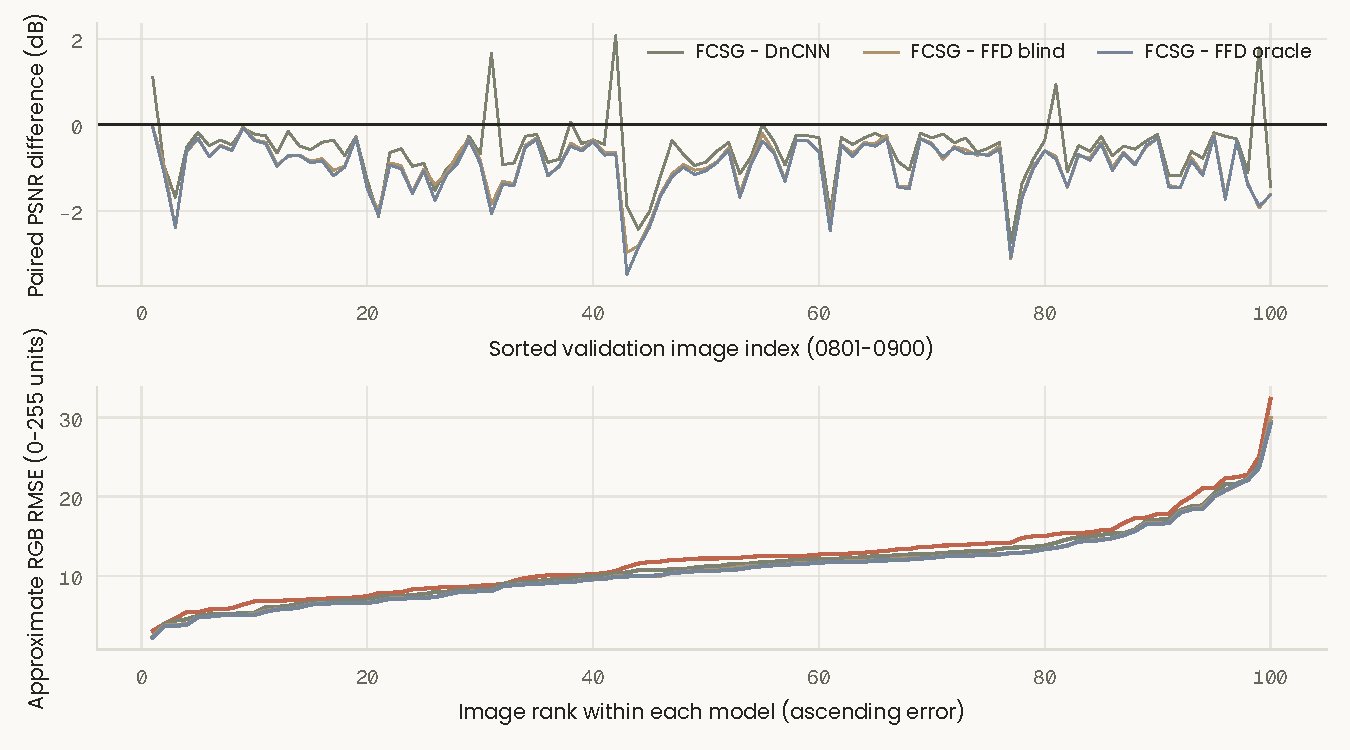
\includegraphics[width=\linewidth]{per_image_errors.pdf}
	\caption{Left: per-image PSNR difference between \fcsg{} and each baseline.
	Right: sorted per-image RMSE for every model (in 8-bit units).}
	\label{fig:per-image}
\end{figure}

\section{Qualitative Results}\label{sec:qualitative}

Figures~\ref{fig:qual-a} and~\ref{fig:qual-b} show the top-left
$320\times320$ region of validation images 0801 and 0802 for each model.
Every model receives the identical degraded input. PSNR labels refer to the
whole image, not the displayed region.

\begin{figure}[htbp]
	\centering
	\begin{subfigure}{\linewidth}
		\centering
		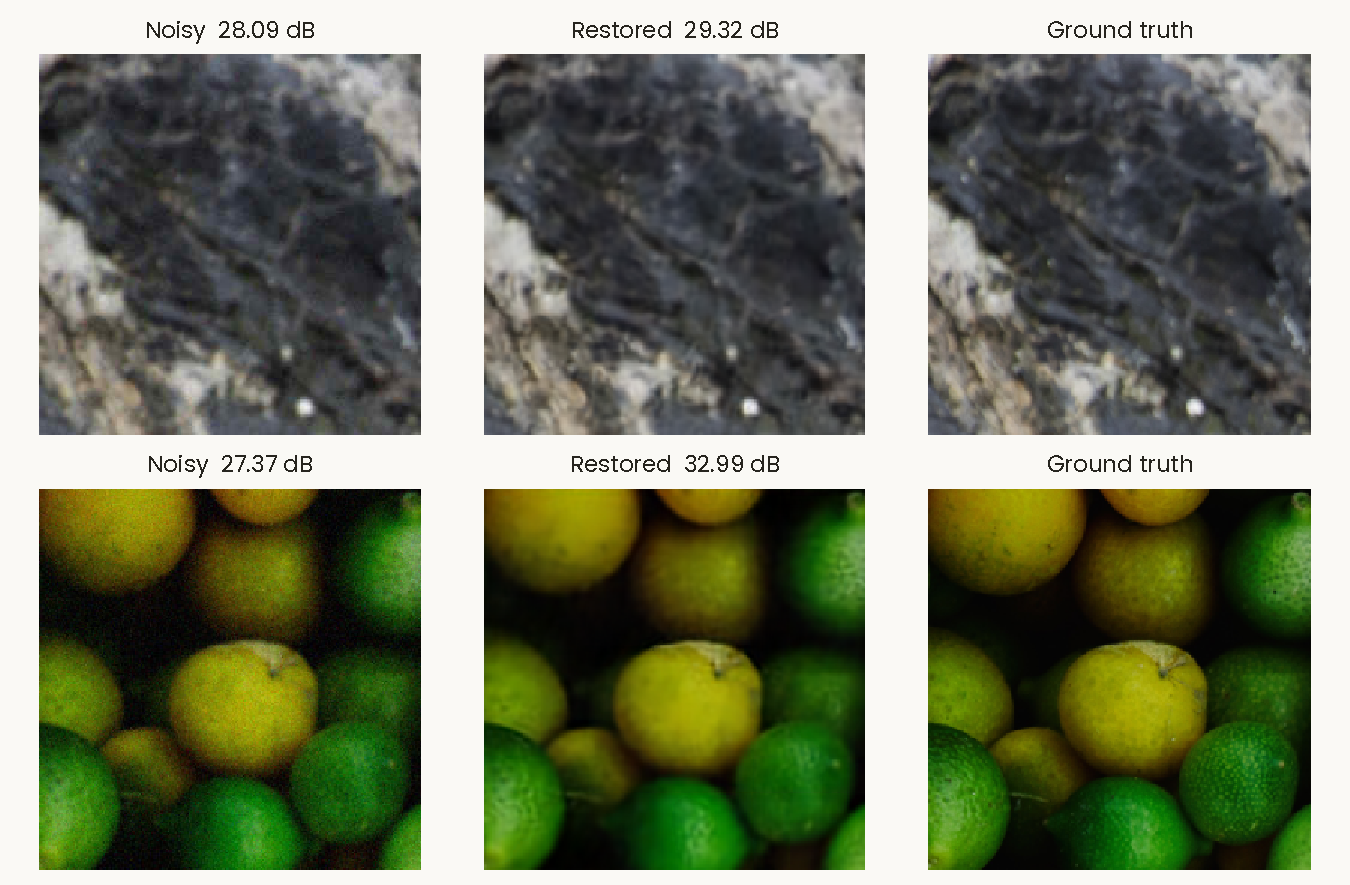
\includegraphics[width=0.92\linewidth]{qualitative_fcsg.pdf}
		\caption{\fcsg{}}
	\end{subfigure}\\[1ex]
	\begin{subfigure}{\linewidth}
		\centering
		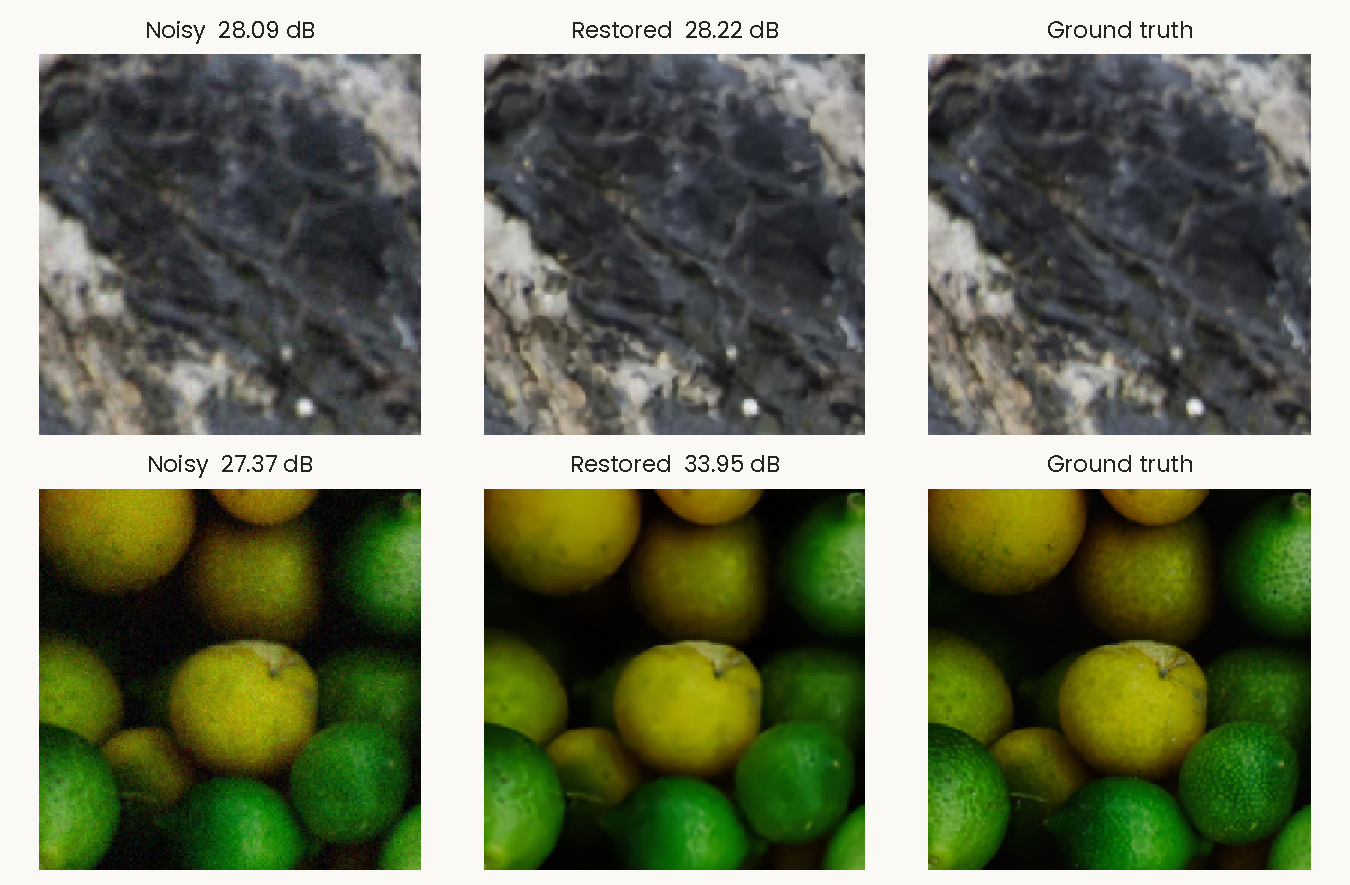
\includegraphics[width=0.92\linewidth]{qualitative_dncnn.pdf}
		\caption{DnCNN}
	\end{subfigure}
	\caption{Degraded input, restoration and clean target for \fcsg{} and DnCNN.}
	\label{fig:qual-a}
\end{figure}

\begin{figure}[htbp]
	\centering
	\begin{subfigure}{\linewidth}
		\centering
		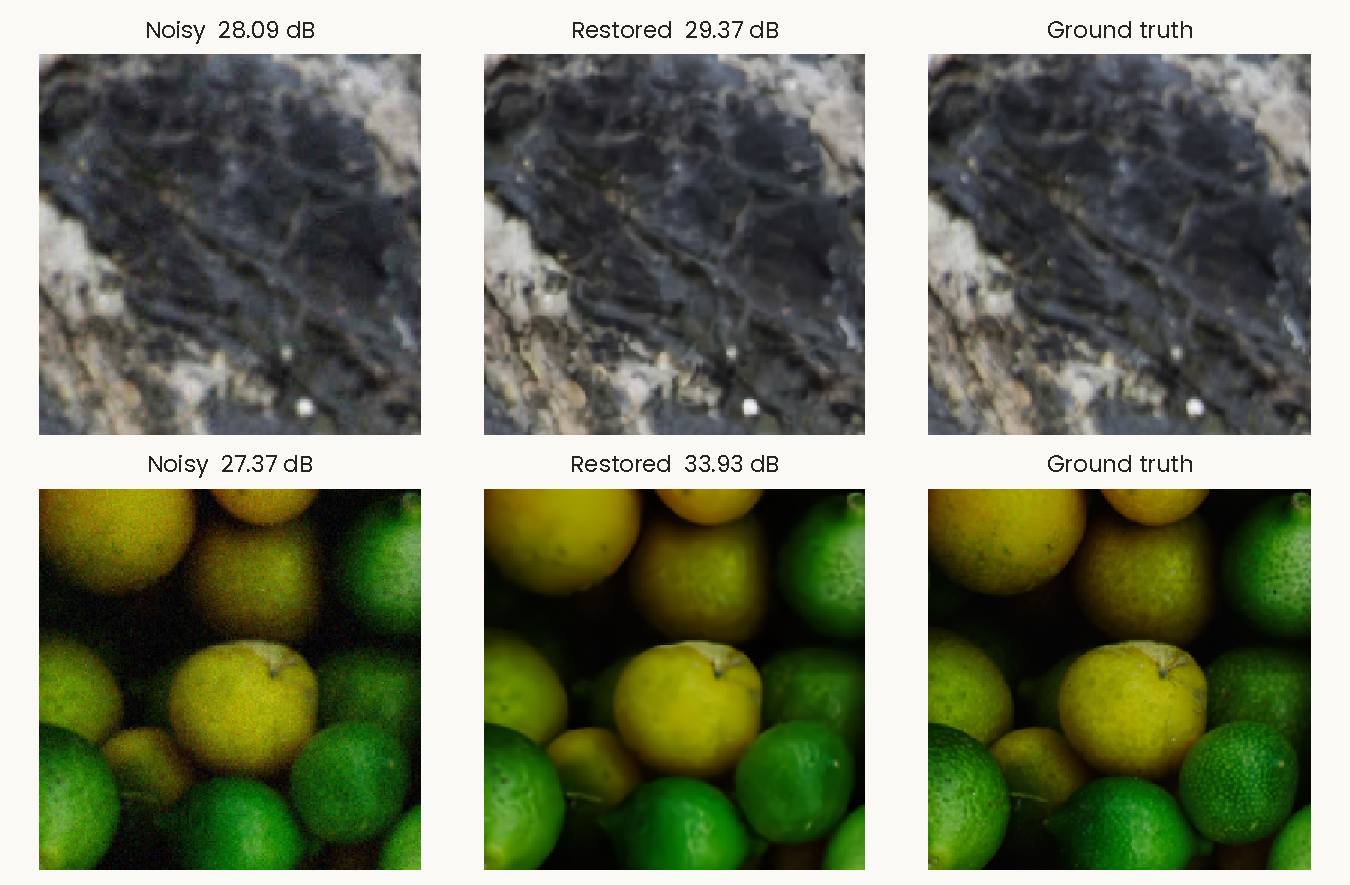
\includegraphics[width=0.92\linewidth]{qualitative_blind.pdf}
		\caption{FFDNet, blind ($\sigma$ map fixed at 27.5/255)}
	\end{subfigure}\\[1ex]
	\begin{subfigure}{\linewidth}
		\centering
		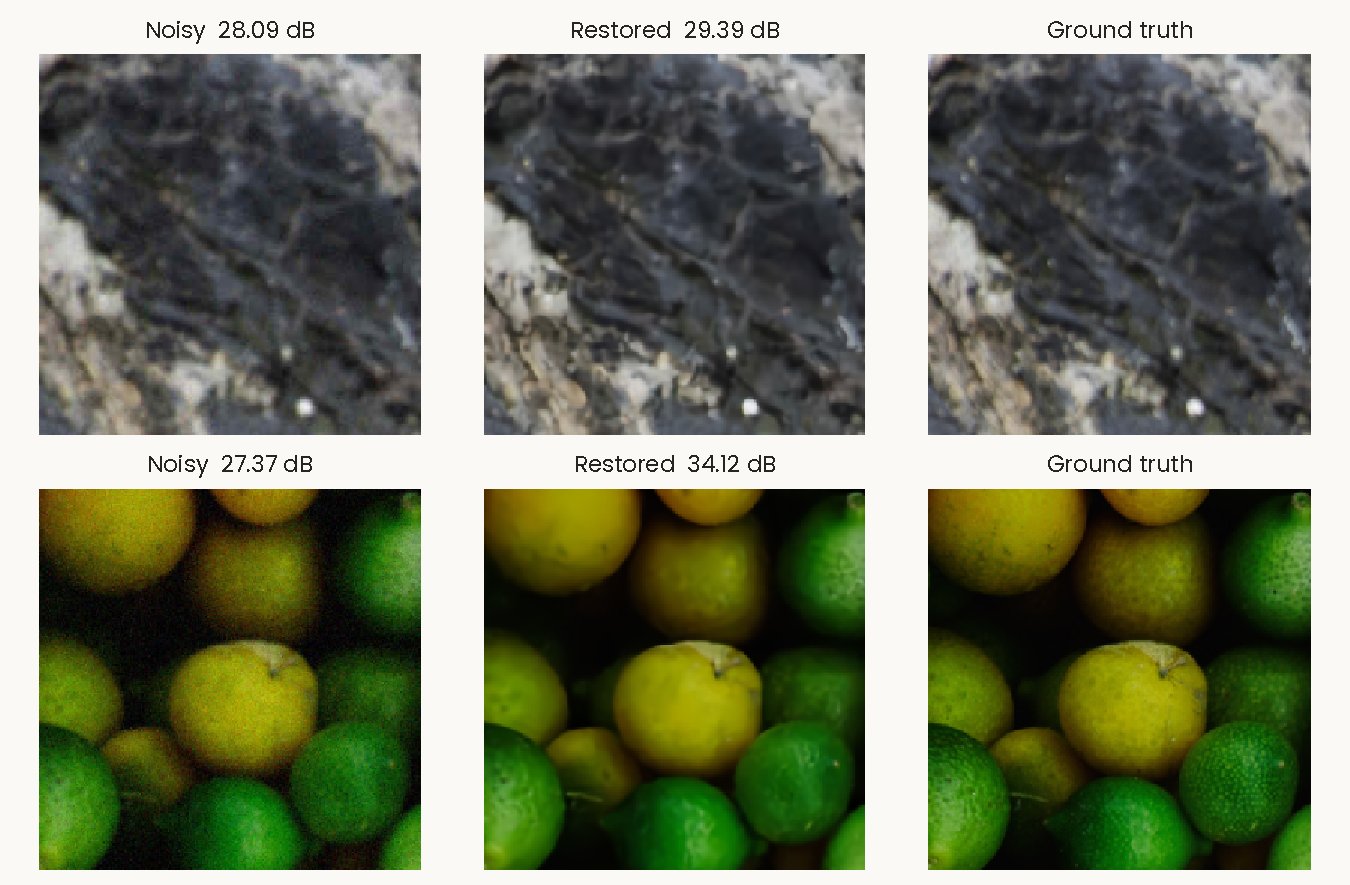
\includegraphics[width=0.92\linewidth]{qualitative_oracle.pdf}
		\caption{FFDNet, oracle (true $\sigma$ map)}
	\end{subfigure}
	\caption{Degraded input, restoration and clean target for the two FFDNet variants.}
	\label{fig:qual-b}
\end{figure}

All four models remove most of the noise and blocking. None of them recovers
the fine texture that blur and downsampling destroyed, which is expected:
those details are not in the input, and a model trained with pixel losses
predicts a smooth average rather than inventing texture. Differences between
models at this scale are subtle, and the saved panels do not include
difference images, so we rely on the quantitative results above rather than
on visual judgement.

\section{Training Convergence}\label{sec:convergence}

Figure~\ref{fig:convergence} plots validation PSNR on the 16 fixed crops
against both updates and wall-clock training time. All four models are close
to a plateau by the end of training. \fcsg{} finishes at 30.59\dB{} on the
crops, below DnCNN (31.66), blind FFDNet (31.97) and oracle FFDNet (32.05),
the same ordering as the full evaluation. Because the curves have flattened,
we have no evidence that simply training \fcsg{} for longer with the same
configuration would close the gap.

\begin{figure}[htbp]
	\centering
	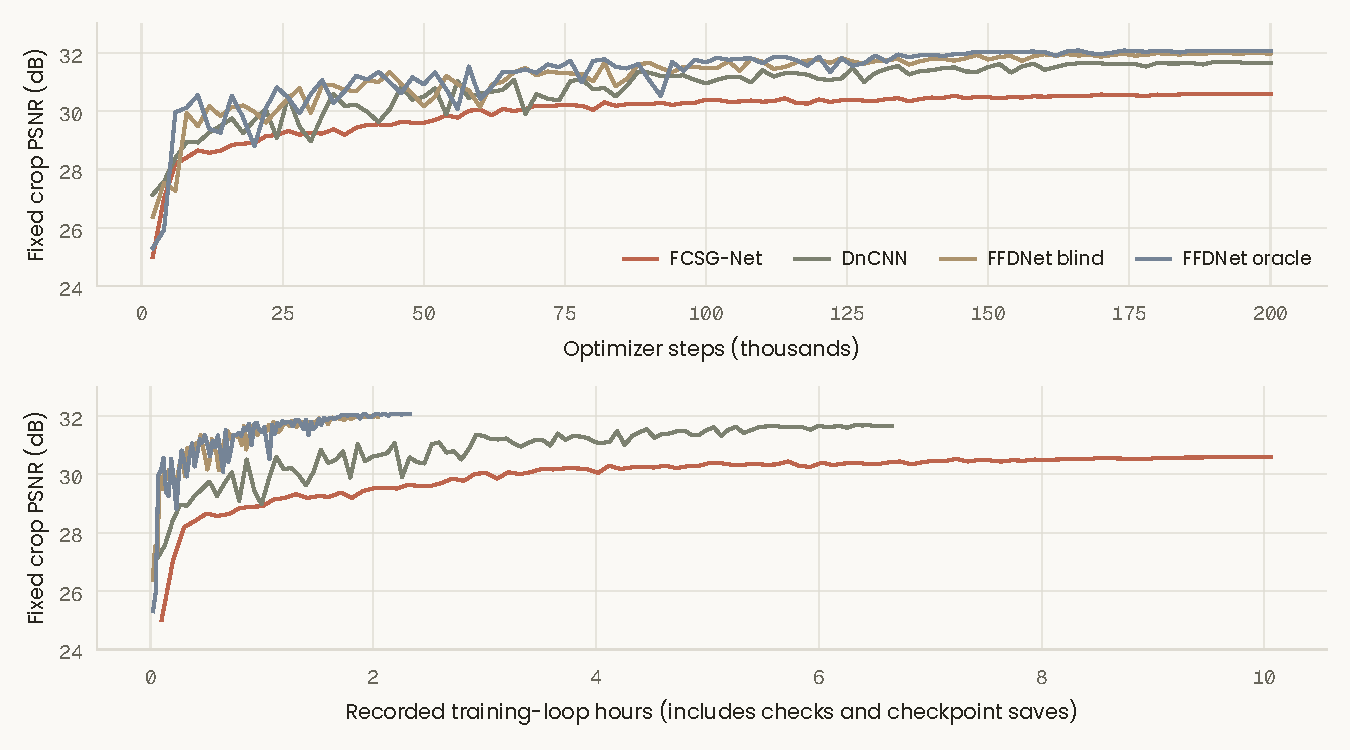
\includegraphics[width=\linewidth]{convergence.pdf}
	\caption{Validation PSNR on 16 fixed crops against updates and training
	time. Crop PSNR is not comparable with the full-image results.}
	\label{fig:convergence}
\end{figure}

The wall-clock panel exposes a cost that the update count hides. \fcsg{}
needed 10.06 hours for 200,000 updates, against 6.66 for DnCNN and about two
for FFDNet. A separate throughput test, excluding warm-up, validation and
checkpointing, measured 5.84 steps per second for \fcsg{}, 9.41 for DnCNN
and 26.67 for FFDNet. Matching the number of updates therefore did not match
the GPU time, and \fcsg{} received the most of it.

\section{Latency, Memory and Tiling}\label{sec:latency}

\paragraph{Latency.} The motivation for a small model is that it should be
cheap to run. Table~\ref{tab:latency} shows that, on the GPU we used, this
did not hold. Measurements are median wall-clock times for one FP32 forward
pass at batch size 1 on a Tesla T4, with TF32 disabled, after 20 warm-up
passes and over 50 timed repetitions.

\begin{table}[htbp]
	\centering
	\caption{Median forward latency (ms) by input size and peak inference memory at $256\times256$ (Tesla T4, FP32, batch 1).}
	\label{tab:latency}
	\begin{tabular}{@{}lrrrr@{}}
		\toprule
		Method & $128^2$ & $256^2$ & $512^2$ & Peak MB at $256^2$ \\
		\midrule
		\fcsg{}          & 5.10 & 19.40 & 75.59 & 51.3 \\
		DnCNN            & 4.22 & 18.04 & 72.47 & 37.8 \\
		FFDNet, blind    & 1.69 &  6.30 & 24.12 & 20.2 \\
		FFDNet, oracle   & 1.69 &  6.35 & 24.62 & 20.2 \\
		\bottomrule
	\end{tabular}
\end{table}

\fcsg{} is the slowest model at every size, slightly behind DnCNN and three
times slower than FFDNet, despite needing an eighth of DnCNN's reported FLOPs
and a third of FFDNet's. It also uses the most memory. We did not profile
individual operators, so the following explanation is our best reading of the
architecture rather than a measurement. Each forward pass runs nine expert
passes, all of them in full, because zero-weighted experts are not skipped.
Depthwise convolutions perform very little arithmetic per byte they read, so
on a GPU their running time is governed by memory traffic, not by the FLOP
count. The network is also made of many small layers, so kernel launch
overhead is a large fraction of the total, and the FFT and inverse FFT add
work that the FLOP estimate counts only approximately. FFDNet, by contrast,
runs one stack of dense $3\times3$ convolutions at half resolution, which is
exactly the kind of workload GPUs are built for.

The practical lesson is that the FLOP budget we set at the start of the
project was the wrong proxy for speed on this hardware. Figure~\ref{fig:cost}
plots quality against both measures. Against FLOPs, \fcsg{} sits far to the
left of the other models. Against latency it sits to the right of FFDNet with
lower quality, so on a T4 it is dominated. Whether the picture changes on a
CPU or a mobile accelerator, where depthwise convolutions are better suited,
remains to be tested.

\begin{figure}[htbp]
	\centering
	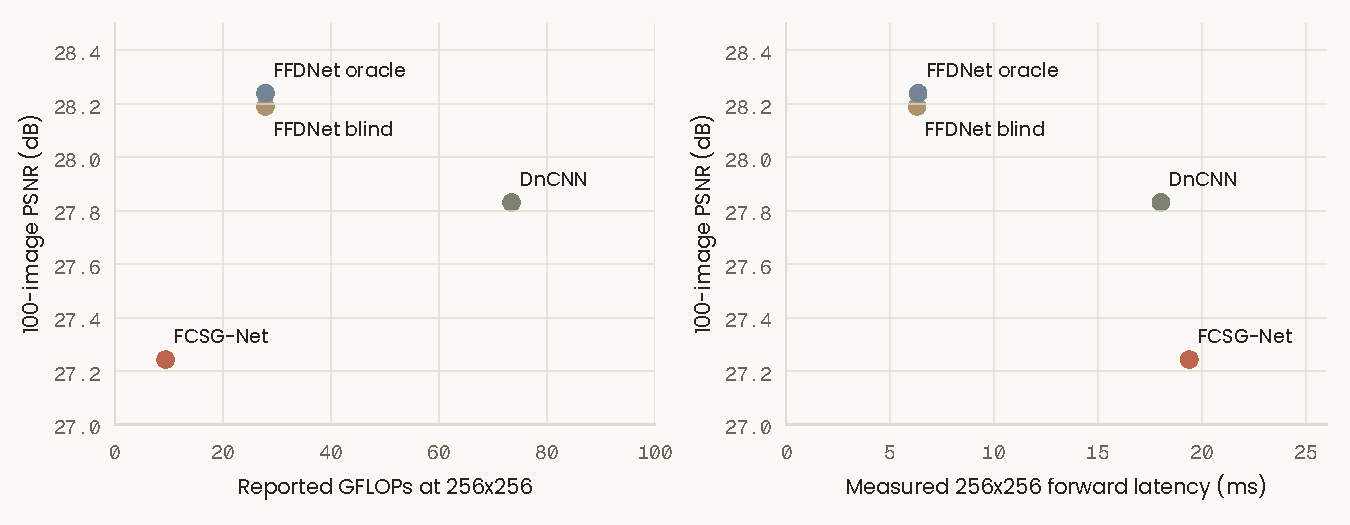
\includegraphics[width=\linewidth]{compute_latency.pdf}
	\caption{Validation PSNR against reported GFLOPs (left) and measured
	$256\times256$ forward latency (right).}
	\label{fig:cost}
\end{figure}

\paragraph{Tiling.} Tiled inference changes what each model sees: the FFT,
the gate's pooling windows and the global pooling in the fusion block all
operate on a $256\times256$ tile rather than the whole image. To measure the
effect we evaluated ten fixed validation images (0801, 0812, \dots, 0900)
with tile sizes of 128, 256 and 512 pixels and a fixed 32-pixel overlap
(Table~\ref{tab:tiling}).

\begin{table}[htbp]
	\centering
	\caption{Mean PSNR (dB) on ten validation images for three tile sizes, 32-pixel overlap.}
	\label{tab:tiling}
	\begin{tabular}{@{}lrrr@{}}
		\toprule
		Method & Tile 128 & Tile 256 & Tile 512 \\
		\midrule
		\fcsg{}         & 26.622 & 26.659 & 26.672 \\
		DnCNN           & 27.330 & 27.341 & 27.343 \\
		FFDNet, blind   & 27.696 & 27.714 & 27.721 \\
		FFDNet, oracle  & 27.730 & 27.748 & 27.756 \\
		\bottomrule
	\end{tabular}
\end{table}

\fcsg{} is the most sensitive to tile size, as expected for a model with
global operations, but the effect is small: going from 256 to 512 pixel
tiles gains 0.013\dB{}, against 0.002\dB{} for DnCNN and about 0.008\dB{}
for FFDNet. This is two orders of magnitude smaller than the 0.6 to 1.0\dB{}
gap in Table~\ref{tab:main}, so tiling does not explain the deficit. The
ten-image means are lower than the 100-image means because the subset
happens to contain harder images; they should be compared only with each
other. Figure~\ref{fig:tiling} shows the paired differences.

\begin{figure}[htbp]
	\centering
	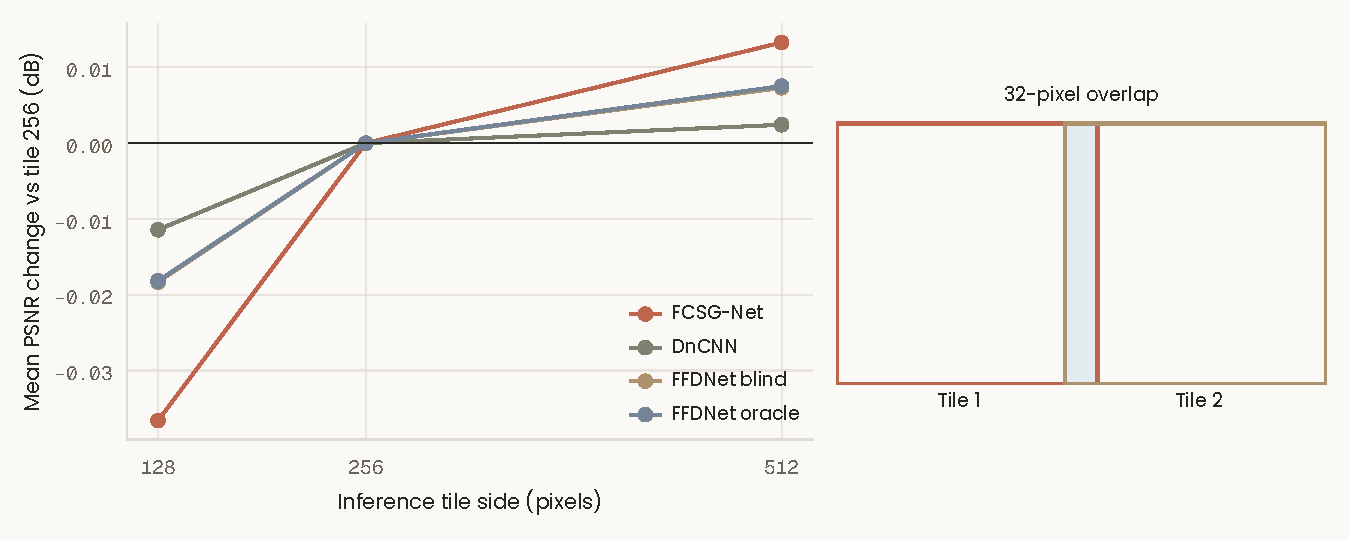
\includegraphics[width=\linewidth]{tiling.pdf}
	\caption{Tile-size sensitivity: PSNR change relative to 256-pixel tiles, and
	the tile and overlap geometry.}
	\label{fig:tiling}
\end{figure}
